\chapter{Bedienungsanleitung}

    \section{Öffnen des Projektes}
        Zunächst wird \textit{Quartus Prime Lite} gestartet.
        Sobald das Hauptfenster geöffnet wurde kann über den Menüpunkt \textit{File}
        der Untermenüpunkt \textit{Open Project} (Abbildung \ref{fig:quartus_open_project})
        geklickt werden. Daraufhin öffnet sich ein Dateibrowser (Abbildung \ref{fig:quartus_select_project})
        durch den das Projekt ausgewählt werden kann.
        Der relative Pfad des Projektes im Repository ist dabei \textit{RiscV-i32/CPU/Design/RiscV.qpf}
        
        \begin{figure}[H]
            \centering
            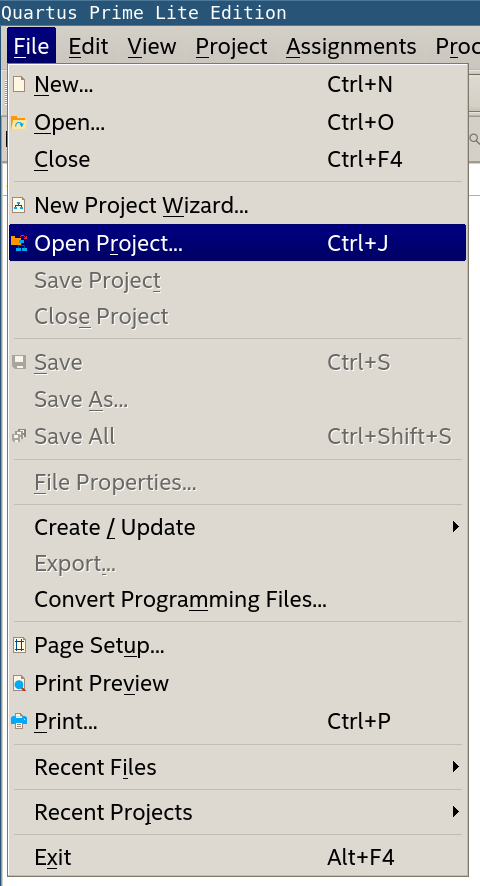
\includegraphics[scale=0.6]{img/quartus_open_project.png}
            \caption{Öffnen des Projektes in Quartus}
            \label{fig:quartus_open_project}
        \end{figure}

        \begin{figure}[H]
            \centering
            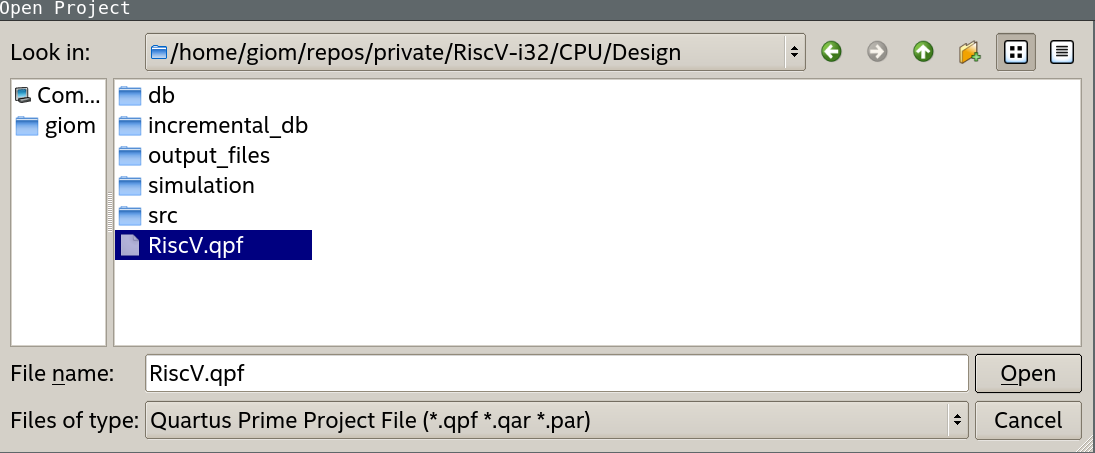
\includegraphics[scale=0.6]{img/quartus_select_project.png}
            \caption{Öffnen des Projektes in Quartus}
            \label{fig:quartus_select_project}
        \end{figure}


    \section{Bauen des Projektes}
        Sobald sich das Projekt erfolgreich geöffnet hat, kann das Bauen über ein Klick
        auf das \textit{Play}-Symbol (Abbildung \ref{fig:quartus_play}) gestartet werden. Das eigentliche Bauen kann, je nach
        Leistung des Rechners mehrere Minuten dauern. Dabei wird der Status im unteren
        Fensterdrittel angezeigt. War das Bauen erfolgreich wird die Meldung
        \textit{Quartus Prime Full Compilation was successful} (Abbildung \ref{fig:quartus_build_sucessful})
        angezeigt.

        \begin{figure}[H]
            \centering
            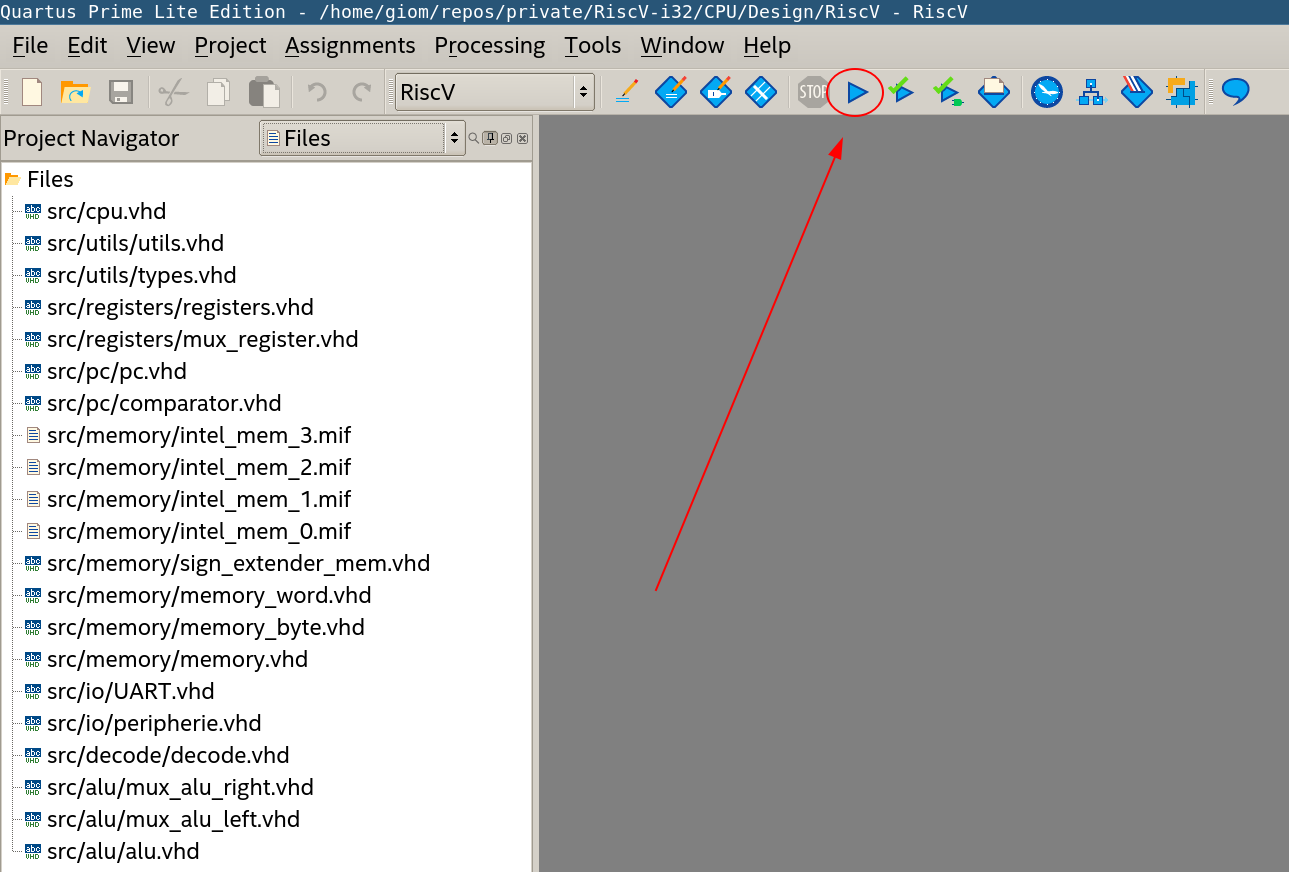
\includegraphics[scale=0.6]{img/quartus_build.png}
            \caption{Bauen des Projektes in Quartus}
            \label{fig:quartus_play}
        \end{figure}

        \begin{figure}[H]
            \centering
            
\includegraphics[scale=0.6]{img/quartus_build_sucessfull.png}
            \caption{Erfolgreiches Bauen des Projektes in Quartus}
            \label{fig:quartus_build_sucessful}
        \end{figure}


    \section{Flashen des FPGAs}\label{lab:flash-fpga}

    Zunächst muss das FPGA-Board über USB angeschlossen werden. Zusätzlich muss der Treiber installiert sein.
    Ist dies der Fall kann über den Menüpunkt \textit{Tools} der Untermenüpunkt \textit{Programmer}
    ausgewählt werden (Abbildung \ref{fig:quartus_programmer}).
    Dadurch öffnet sich der Programmer (Abbildung \ref{fig:quartus_programmer_window})
    und die Hardware kann durch einen Klick auf \textit{Hardware Setup} eingerichtet werden.
    Ein weiteres Fenster öffnet sich (Abbildung \ref{fig:quartus_programmer_select_hardware}).
    Ein Doppelklick auf \textit{Arrow-USB-Blaster (1)} wählt das FPGA-Board als Ziel für den Programmer.
    Dies kann durch \textit{Currently selected Hardware (2)} bestätigt werden. Ein weiterer Klick auf
    \textit{close} schließt das Fenster wieder. Nun kann über \textit{Start}
    (Abbildung \ref{fig:quartus_programmer_start}) das eigentliche Flashen beginnen.
    Eine visuelle Rückmeldung bietet hierbei der Ladebalken \textit{Progress}.
    

    \begin{figure}[H]
        \centering
        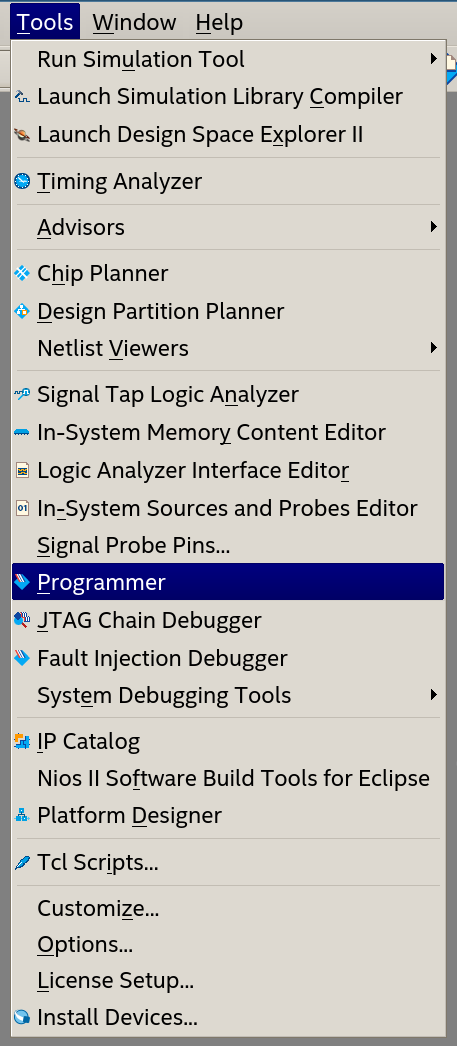
\includegraphics[scale=0.6]{img/quartus_programmer.png}
        \caption{Öffnen des Programmers in Quartus}
        \label{fig:quartus_programmer}
    \end{figure}

    \begin{figure}[H]
        \centering
        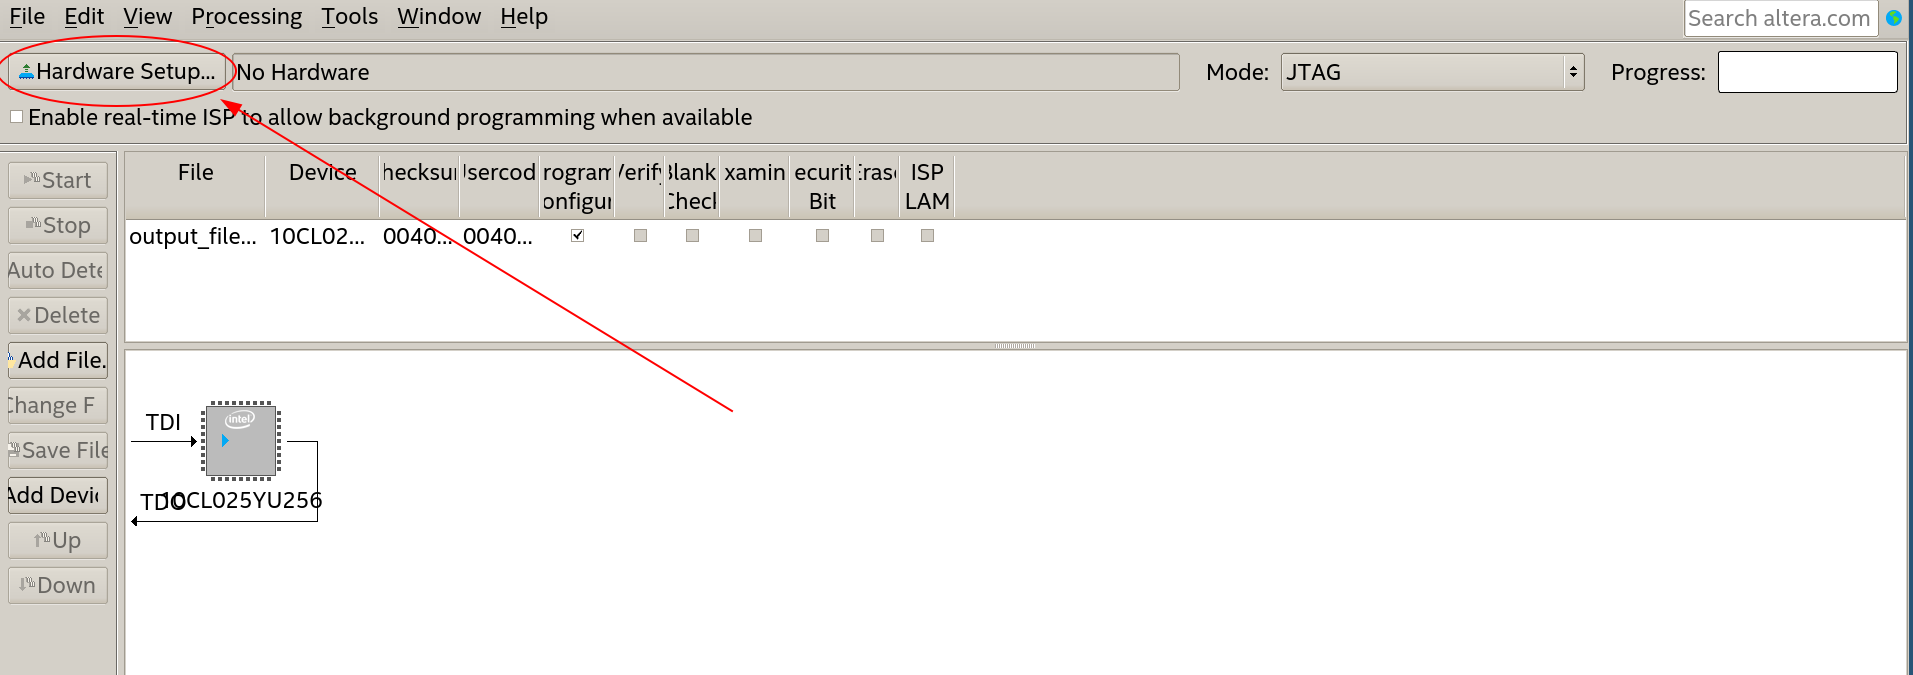
\includegraphics[scale=0.6]{img/quartus_programmer_select_hardware.png}
        \caption{Einrichten der Hardware in Quartus}
        \label{fig:quartus_programmer_window}
    \end{figure}

    \begin{figure}[H]
        \centering
        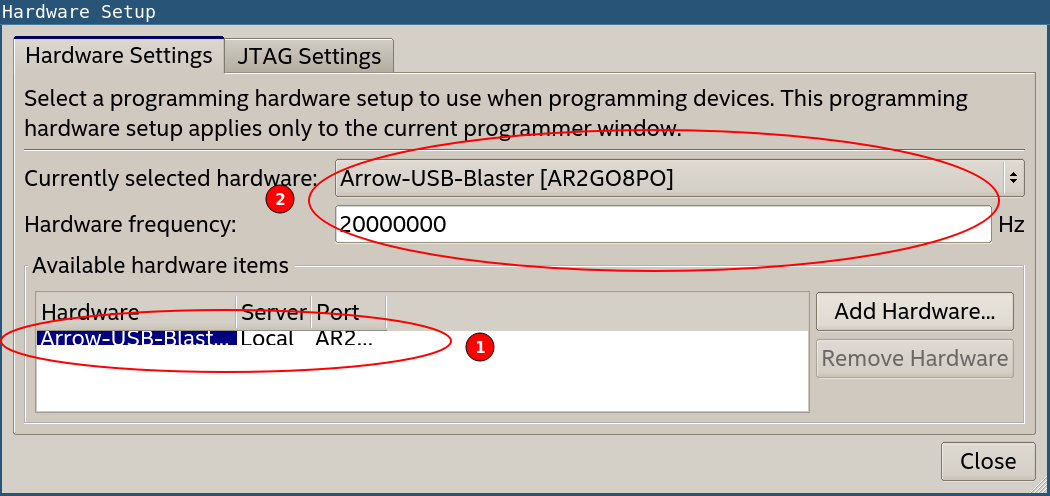
\includegraphics[scale=0.6]{img/quartus_programmer_select_hardware2.png}
        \caption{Einrichten der Hardware in Quartus}
        \label{fig:quartus_programmer_select_hardware}
    \end{figure}

    \begin{figure}[H]
        \centering
        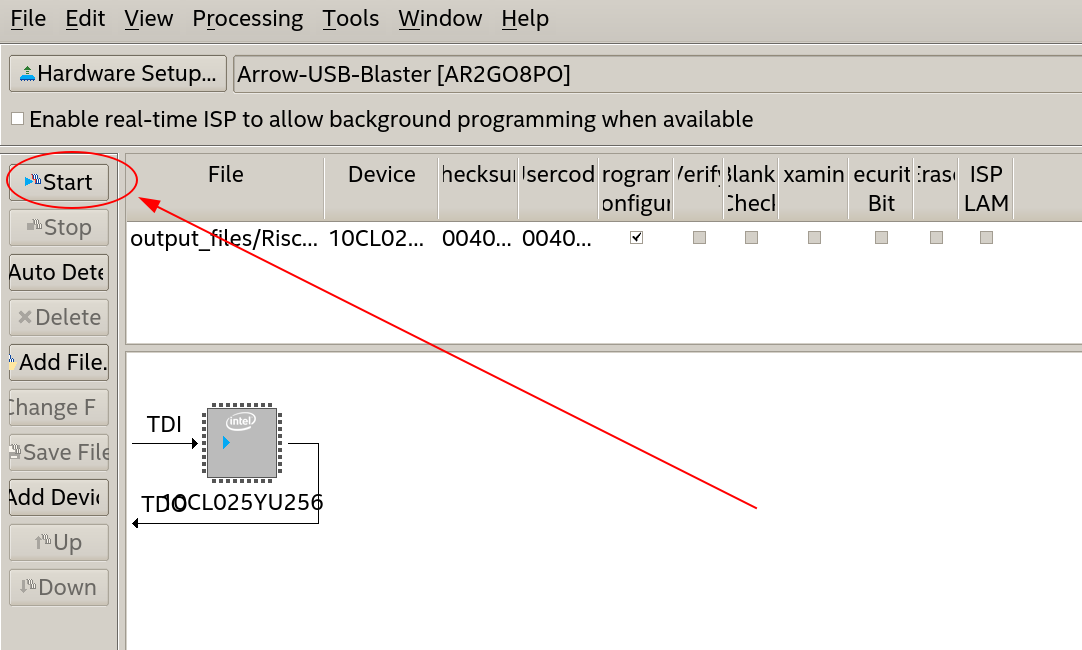
\includegraphics[scale=0.6]{img/quartus_programmer_start.png}
        \caption{Starten des Flashens des FPGAs}
        \label{fig:quartus_programmer_start}
    \end{figure}


    \section{Kompilieren des Programmcodes}\label{lab:compile-code}
        Um Programmcode zu Compilieren muss zunächst die Toolchain gebaut werden
        dessen Quellcode sich im \textit{Firmware} Verzeichnis befindet.
        Nach wechseln in das Verzeichnis kann über den Befehl \texttt{go build *.go}
        die Toolchain gebaut werden. War das bauen Erfolgreich erscheint
        eine ausführbare Datei namens \textit{build} im Verzeichnis.
        Durch \texttt{./build --help} wird die Parameterübersicht des Programmes
        ausgegeben (Abbildung \ref{fig:build-help}).

        \begin{figure}[H]
            \centering
            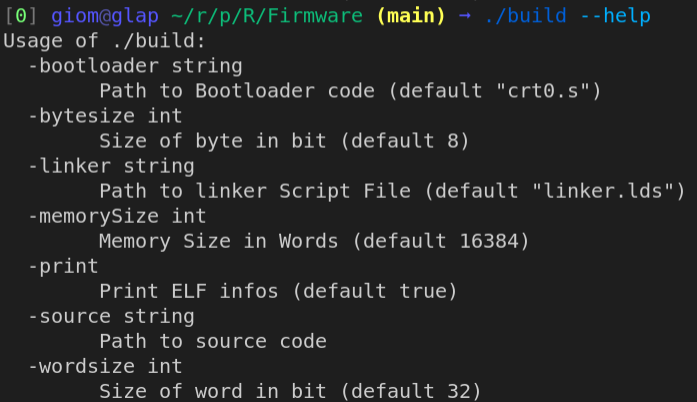
\includegraphics[scale=1]{img/build_help.png}
            \caption{Parameterübersicht von Build}
            \label{fig:build-help}
        \end{figure}
        Die Standardbelegung der Parameter ist auf die hardware Eigenschaften des
        Softcores ausgelegt, sodass nur \texttt{./build --source=PFAD} benötigt wird
        um das jeweilige Programm zu Compilieren.
        \\
        Zum testen des Bauprozesses befindet sich Beispielquellcode im
        \textit{src} Verzeichnis.
        Beispielsweise kann über \texttt{./build --source=src/lightshift.c}
        ein einfaches Programm Compiliert werden. Da der \textit{Print}-Parameter
        standardmäßig auf \textit{true} gesetzt ist, werden nach Erfolgreichem
        compilieren die Partitionstabellen sowie der assemblierte Programmcode
        ausgegeben (Abbildung \ref{fig:build-example}).


        \begin{figure}[H]
            \centering
            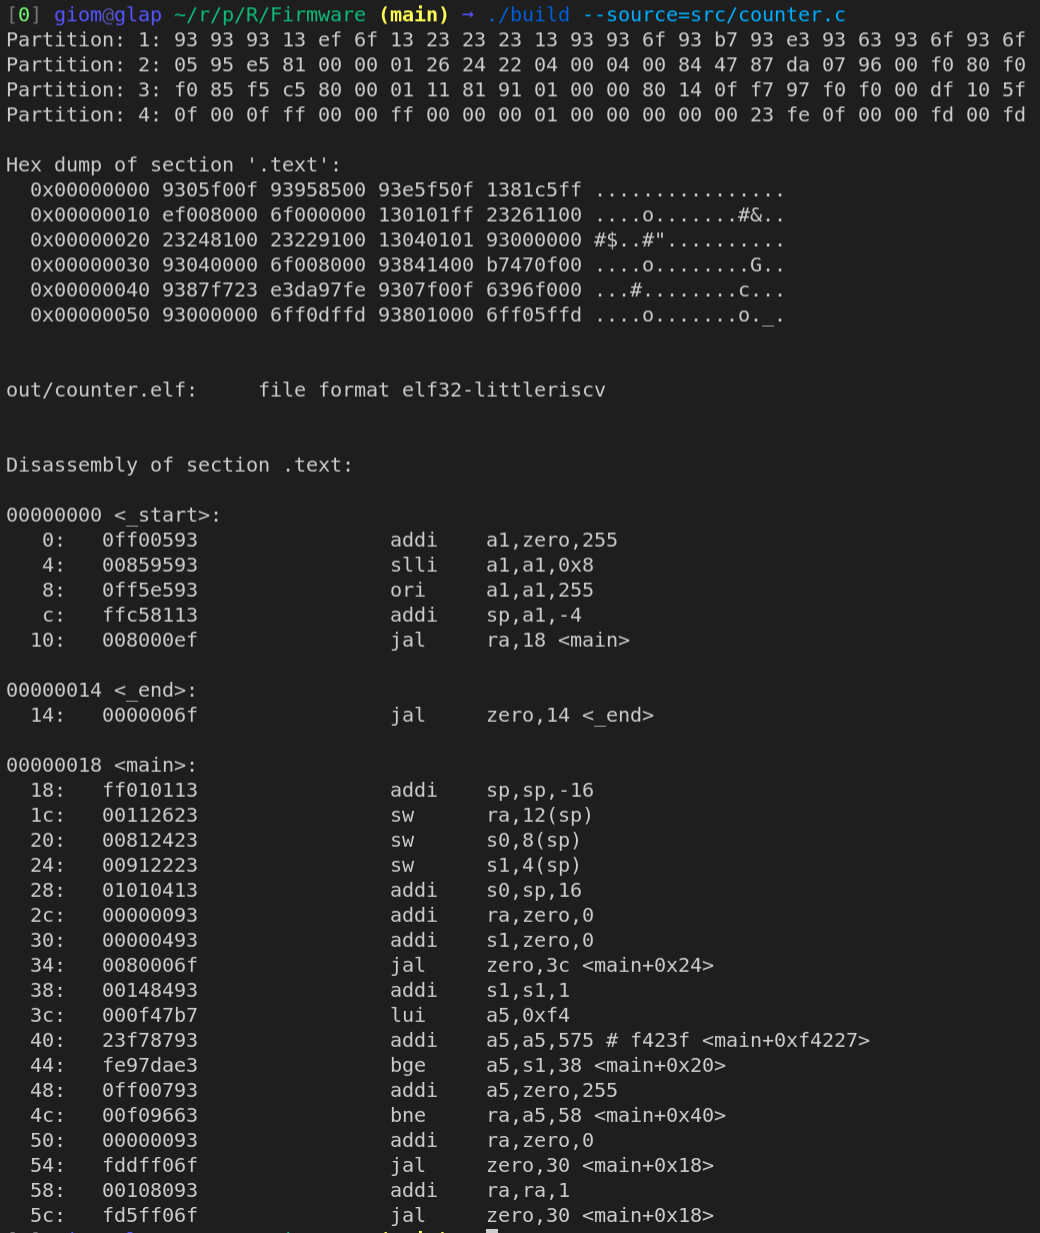
\includegraphics[scale=1]{img/build_example.png}
            \caption{Beispielquellcode compiliert durch build}
            \label{fig:build-example}
        \end{figure}

        \subsection{Plattform.h}
            Der Zugriff auf die Peripherie wird über \textit{Memory-Mapping} realisiert.
            Die Adressen sind hierfür in der \textit{Plattform.h} im \textit{src}-Verzeichnis
            hinterlegt (Listing \ref{lst:plattformh}).
            \lstinputlisting[style=cstyle,caption={Plattform.h},label=lst:plattformh]{../../Firmware/src/plattform.h}
            Die Bedienung der Peripherie erfolgt aus dem Programmcode wie im Beispiel von \textit{lightshift.c} (Listing \ref{lst:ligthshiftc}).
            \lstinputlisting[style=cstyle,caption={Ligthshift.c},label=lst:ligthshiftc]{../../Firmware/src/lightshift.c}

    \section{Flashen des Softcores}

        Zunächst müssen die generierten \textit{MIFs} aus dem \textit{out} Verzeichnis in
        \textit{RISC-V/CPU/Design/src/memory} kopiert werden.
        Als nächstes wird über den den Menüpunkt \textit{Processing},
        \textit{Update Memory Initialization File} angeklickt (Abbildung \ref{fig:update-mif}).
        Daraufhin muss im selben Menüpunkt das Untermenü \textit{Start} geöffnet werden um
        \textit{Start Assembler} anzuklicken (Abbildung \ref{fig:start-asm}).
        Als letztes muss der FPGA erneut geflashed werden (Siehe \ref{lab:flash-fpga}).
        Dabei wird jedoch nur der letzte Schritt benötigt (Abbildung \ref{fig:quartus_programmer_start}).


        \begin{figure}[H]
            \centering
            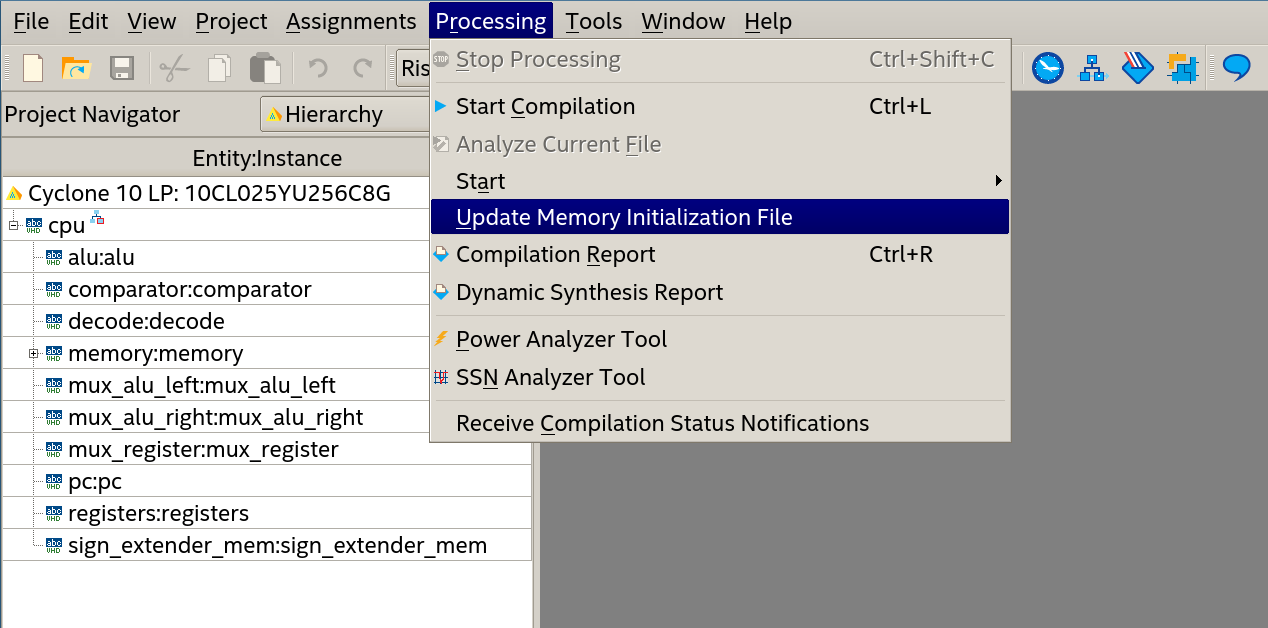
\includegraphics[scale=0.6]{img/update_mif.png}
            \caption{MIF Aktualisieren}
            \label{fig:update-mif}
        \end{figure}

        \begin{figure}[H]
            \centering
            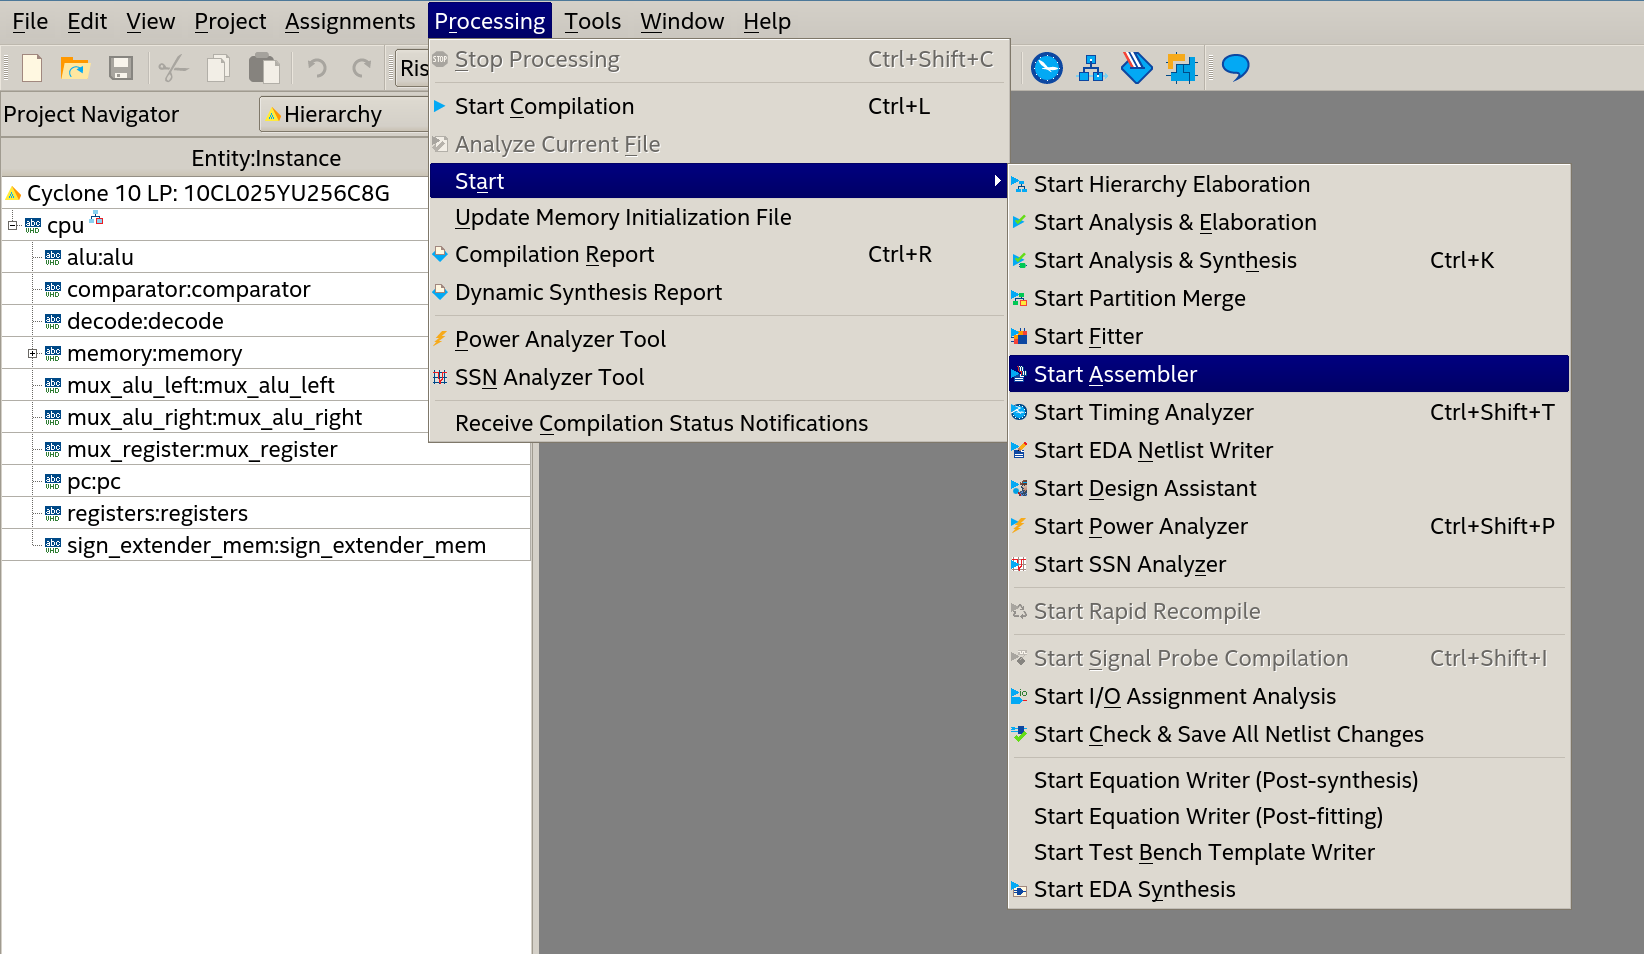
\includegraphics[scale=0.5]{img/start_assembler.png}
            \caption{Assemblierung}
            \label{fig:start-asm}
        \end{figure}

